\documentclass[xcolor=table]{beamer}
\mode<presentation>
\usetheme{CambridgeUS}
\usepackage[russian]{babel}
\usepackage[utf8]{inputenc}
\usepackage[T2A]{fontenc}
\usepackage{sansmathaccent}
\usepackage{verbatim}
\usepackage{alltt}
\usepackage[table]{xcolor}
%\linespread{0.8}
\usepackage{minted}
\usepackage{setspace}

\pdfmapfile{+sansmathaccent.map}
\title[Файловая система]{Файловая система в Linux}
\author{Наумов Д.А., доц. каф. КТ}
\date[29.10.2019] {Операционные системы и системное программное обеспечение, 2019}

\begin{document}

%ТИТУЛЬНЫЙ СЛАЙД
\begin{frame}
  \titlepage
\end{frame}
  
%СОДЕРЖАНИЕ ЛЕКЦИИ
\begin{frame}
  \frametitle{Содержание лекции}
  \tableofcontents  
\end{frame}

\section{Обзор файловой системы в Linux}
	
\begin{frame}{Аксиоматика файловой системы в Linux}
	Типичная модель файловой системы Linux:
	\begin{itemize}
		\item \textbf{нижний уровень}: драйверы устройств и файловых систем, полностью реализован в ядре Linux.
		\item \textbf{cредний уровень}: системные вызовы, работающие с файловыми системами и осуществляющие низкоуровневый ввод-вывод, унифицированный интерфейс файловой системы, семь типов файлов (<<everything is file>>): 
		\begin{enumerate}
			\item каталоги, 
			\item символьные устройства, 
			\item блочные устройства,
			\item обычные файлы, 
			\item каналы FIFO, 
			\item символические ссылки,
			\item сокеты.
		\end{enumerate}
		\item верхний уровень: библиотеки и приложения, которые создают полноценную иллюзию единого дерева файловой системы.
	\end{itemize}
\end{frame}

\begin{frame}[fragile]{Типы файлов. Обычный файл}
	\begin{block}{Обычный файл (file)}
		обозначенная некоторым именем последовательность данных, которые хранятся на диске (устройстве хранения данных).
	\end{block}
	\begin{block}{Создадим пустой файл при помощи программы \textit{touch}:}
		\begin{alltt}
			\$ touch anyfile
		\end{alltt}
	\end{block}
	\begin{block}{Теперь наберем следующую команду:}
		\begin{alltt}
			\$ ls -l anyfile

			-rw-r--r-- 1 nnivanov nnivanov 0 2011-05-06 20:11 anyfile
		\end{alltt}
	\end{block}
	Прочерк в самом начале -- поле типа файла с точки зрения среднего уровня реализации файловой системы. \textit{Если здесь стоит минус, то это обычный файл}.
\end{frame}

\begin{frame}[fragile]{Типы файлов. Каталог}
	\begin{block}{Каталог (директория, directory)}
		формально тоже считается файлом, содержащим данные о файлах, хранящихся в нем.
	\end{block}
	\begin{block}{Давайте теперь создадим каталог:}
		\begin{alltt}
			\$ mkdir anydir
			\$ ls -l

			drwxr-xr-x 2 nnivanov nnivanov 4096 2011-05-06 20:13 anydir/
			-rw-r--r-- 1 nnivanov nnivanov 0 2011-05-06 20:11 anyfile
		\end{alltt}
	\end{block}
	В поле типа файла для \textit{anydir} находится символ \textit{d}, показывающий, что это каталог (\textit{directory}).
\end{frame}

\begin{frame}[fragile]{Типы файлов. Символические ссылки}
	\begin{block}{Символьная или мягкая ссылка (символическая ссылка, symbolic link, simlink)}
		указатель на другой файл, предназначена для исключения дублирования и более оптимального использования места на диске. 
	\end{block}
	\begin{block}{Создадим символическую ссылку:}
		\begin{alltt}
			\$ ln -s anyfile anylink
			\$ ls -l

			drwxr-xr-x 2 nnivanov nnivanov 4096 2011-05-06 20:13 anydir/
			-rw-r--r-- 1 nnivanov nnivanov 0 2011-05-06 20:11 anyfile
			lrwxrwxrwx 1 nnivanov nnivanov 7 2011-05-06 20:14 anylink 
			                                                  -> anyfile
		\end{alltt}
	\end{block}
	Символические ссылки в выводе \textit{ls} обозначаются символом \textit{l} (\textit{link}).
\end{frame}

\begin{frame}[fragile]{Типы файлов. Устройства}
	Устройства в \textit{Linux} могут быть представлены в виде файлов. 
	Файлы устройств отображаются в каталоге \textbf{/dev} дерева каталогов \textit{Linux}.

	На среднем уровне реализации файловой системы под устройствами понимают файлы двух типов:
	\begin{itemize}
		\item символьные устройства, обозначаемые символом \textit{c} (\textit{character});
		\item блочные устройства, обозначаемые символом \textit{b} (\textit{block}).
	\end{itemize}
	Файл устройства не обязательно соответствует какому-либо реальному устройству. Он может соответствовать и виртуальному устройству, реализуемому программно (/dev/random). 
	\begin{block}{Введите следующую команду:}
		\begin{alltt}
			\$ ls -l /dev/null
			crw-rw-rw- 1 root root 1, 3 2011-05-06 20:16 /dev/null
		\end{alltt}
	\end{block}
	Вывод программы ls показывает, что /dev/null является символьным устройством.
\end{frame}

\begin{frame}[fragile]{Устройства}
	На среднем уровне реализации файловой системы все устройства представляются двумя типами файлов:
	\begin{block}{Символьные устройства (character devices)}
		\begin{itemize}
			\item особенность - механизм последовательного ввода-вывода;
			\item рассматриваются не в виде линейного массива данных, а как поток информации.
		\end{itemize}
	\end{block}
	\begin{block}{Блочные устройства (block devices)}
		\begin{itemize}
			\item читают и записывают данные блоками фиксированного размера с использованием механизма буферизации. 
			\item файлы устройств этого типа чаще всего применяются для дисковых накопителей и для дисковых разделов. 
			\item некоторые сетевые устройства также могут быть представлены файлами этого типа.
		\end{itemize}
	\end{block}
\end{frame}

\begin{frame}[fragile]{Типы файлов. Устройства}
	Унификация обозначения устройств, содержащих файловые системы, жесткие диски, USBнакопители, CD/DVD-приводы, SCSI-устройства:
	\begin{block}{Cписок блочных устройств:}
		\begin{alltt}
			\$ ls -l /dev/sd*

			brw-rw---- 1 root disk 8, 0 2011-05-06 18:41 /dev/sda
			brw-rw---- 1 root disk 8, 1 2011-05-06 18:41 /dev/sda1
			brw-rw---- 1 root disk 8, 2 2011-05-06 18:41 /dev/sda2
			brw-rw---- 1 root disk 8, 16 2011-05-06 18:53 /dev/sdb
			brw-rw---- 1 root disk 8, 17 2011-05-06 18:53 /dev/sdb1
		\end{alltt}
	\end{block}
\end{frame}

\begin{frame}[fragile]{Типы файлов. Каналы}
	Для взаимодействия процессов (выполняемых на одной машине) существуют особые файлы, которые называются \textbf{каналами FIFO} (First In First Out) или просто \textbf{FIFO}. 

	\medskip
	Эти файлы создаются командой \textit{mkfifo} и обозначаются в выводе программы \textbf{ls} символом \textbf{p} (\textit{pipe}):
	\begin{block}{Создание канала:}
		\begin{alltt}
			\$ mkfifo anyfifo
			\$ ls -l anyfifo

			prw-r--r-- 1 nnivanov nnivanov 0 2011-05-06 20:33 anyfifo
		\end{alltt}
	\end{block}
\end{frame}

\begin{frame}[fragile]{Типы файлов. Сокеты}
	\textbf{Сокет} (socket) похож на канал в том смысле, что тоже является механизмом для обмена данными между двумя разными процессами. Однако
сокет имеет два важных отличия от канала:
	\begin{itemize}
		\item процессы чаще всего запущены на разных компьютерах;
		\item обмен данными осуществляется по сети с использованием стека протоколов \textit{TCP/IP}.	
	\end{itemize}

	\medskip
	Сокеты обозначаются в выводе команды \textit{ls} символом \textit{s} (socket). 

	\medskip	
	\textbf{Сокеты }динамически создаются программами при помощи системного вызова \textit{socket()}. 
\end{frame}

\begin{frame}[fragile]{Права доступа}
	В Linux каждый файл имеет своего \textbf{владельца} (и только одного) - им обычно является пользователь, создавший этот файл.

	\medskip
	Владелец файла определяет \textbf{права доступа} к файлу. Для каждого файла могут быть заданы: 
	\begin{itemize}
		\item право на чтение;
		\item право на запись;
		\item право на выполнение. 
	\end{itemize}

	Указанные права задаются отдельно для трех категорий пользователей:
	\begin{itemize}
		\item для владельца файла;
		\item для пользователей, входящих в так называемую группу владельца (ограниченный круг доверенных пользователей владельца, которых он сам определяет, включая в группу пользователей, имя которой совпадает с именем владельца);
		\item для всех остальных пользователей.
	\end{itemize}	
\end{frame}

\begin{frame}[fragile]{Права доступа}
	Владельца файла можно посмотреть в расширенном листинге команды \textbf{ls}:

	\begin{alltt}
		\$ ls -l

		-rw-r--r-- 2 user user 132 Мар 23 14:39 file1.txt
		-rw-r--r-- 2 user user 132 Мар 23 14:39 file_hard
		lrwxrwxrwx 1 user user 9 Мар 23 14:40 file_soft -> file1.txt		
	\end{alltt}
\end{frame}

\begin{frame}[fragile]{Права доступа}
	Основные права доступа часто задают в виде трех восьмеричных цифр, например \textbf{764}. 
	\begin{itemize}
		\item первая цифра (7) определяет права владельца файла, 
		\item вторая (6) – права группы владельца, 
		\item третья (4) – права остальных пользователей.
	\end{itemize}
	Каждая восьмеричная цифра прав складывается из трех двоичных разрядов:
	\begin{itemize}
		\item права на исполнение (в разряде единиц), 
		\item права на запись (в разряде двоек) 
		\item права на чтение (в разряде четверок).	
	\end{itemize}
	
	Для каталогов права доступа носят особый смысл:
	\begin{itemize}
		\item право на чтение позволяет просматривать содержимое каталога, 
		\item право на запись позволяет удалять или перемещать файлы в каталоге, 
		\item право на выполнение вместе с правом на чтение – осуществлять поиск в каталоге.
	\end{itemize}	
\end{frame}

\begin{frame}[fragile]{Права доступа}
	\begin{itemize}
		\item Когда процесс пытается получить доступ к какому-нибудь файлу, ядро Linux использует UID текущего процесса для проверки прав доступа.
		\item Если проверка не удалась, в ход идет GID (Group ID, идентификатор группы). 
		\item Если и здесь доступ закрыт, проверяются права доступа для остальных пользователей.
	\end{itemize}
	\begin{block}{Права доступа файла shadow}
		\begin{alltt}
		\$ ls -l shadow

		-r--r----- 1 root shadow 1012 2011-03-08 10:03 /etc/shadow
		\end{alltt}
	\end{block}
	Данные о пользователях хранятся в файле /etc/passwd, который открыт для всех, а зашифрованные пароли находятся в файле /etc/shadow, доступ к которому разрешен только суперпользователю.
\end{frame}

\begin{frame}[fragile]{Права доступа}
	Программ \textbf{su} позволяет временно входить в систему на правах другого пользователя. 

	\textit{Как su "умудряется" сравнивать введенные вами пароли с содержимым закрытого от посторонних глаз файла /etc/shadow? }
	\begin{block}{В первом окне введите команду su:}
		\begin{alltt}
			\$ su
			Password:
		\end{alltt}
	\end{block}
	\begin{block}{Перейдем в другое окно и введем:}
		\begin{alltt}
			\$ ps -ef
			...
			nnivanov 17952 9299 0 20:37 pts/1 00:00:00 bash
			root 17989 9302 0 20:37 pts/0 00:00:00 su
			nnivanov 18008 17952 0 20:37 pts/1 00:00:00 ps -efu
		\end{alltt}
	\end{block}
\end{frame}

\begin{frame}[fragile]{Права доступа}
	\begin{block}{Введите теперь следующую команду:}
		\begin{alltt}
			\$ ls -l /bin/su

			-rwsr-xr-x 1 root root 34500 2010-04-29 19:17 /bin/su
		\end{alltt}
	\end{block}
	\begin{itemize}
		\item Триада, показывающая базовые права доступа для пользователя, содержит символ s на месте бита исполнения. 
		\item Этот символ означает, что для исполняемого файла установлен бит SUID (Set User IDentifier), который позволяет запускать данную 		программу от лица владельца ее исполняемого файла. 
		\item Существует бит SGID (Set Group IDentifier), который позволяет запускать программу от имени группы, которой принадлежит этот файл.
	\end{itemize}
\end{frame}

\begin{frame}[fragile]
	К процессу привязано два идентификатора пользователя:
	\begin{itemize}
		\item реальный UID (Real UID, RUID или просто UID);
		\item эффективный UID (Effective UID или просто EUID).
	\end{itemize}
	В большинстве случаев эти идентификаторы равны. Но если для исполняемого файла программы установлен бит SUID, то ситуация меняется. 
	\begin{block}{Пример}
		когда пользователь anyuser запускает программу su, то реальный UID процесса равен идентификатору пользователя anyuser, а эффективный UID  равен идентификатору пользователя root.
	\end{block}
	\begin{block}{Установить бит SUID для исполняемого файла:}
		\begin{alltt}
			\$ chmod u+s file
		\end{alltt}
	\end{block}
	\begin{block}{Установить бит SGID для исполняемого файла:}
		\begin{alltt}
			\$ chmod g+s file
		\end{alltt}
	\end{block}
\end{frame}

\begin{frame}[fragile]
	Расширенные права доступа позволяют задействовать еще один бит, который называется битом \textbf{SVTX} или \textbf{липким битом} (sticky). 
	
	В каталоге с установленным битом SVTX каждый может создавать, удалять и переименовывать файлы могут только владелец файла и суперпользователь.  
	\begin{block}{Каталог /tmp, доступен всем для хранения временных файлов:}
		\begin{alltt}
			\$ ls -l / | grep tmp

			drwxrwxrwt 63 root root 12288 2011-05-06 20:42 tmp/
		\end{alltt}
	\end{block}
	\begin{block}{Назначить каталогу directory липкий бит:}
		\begin{alltt}
			\$ chmod +t directory
		\end{alltt}
	\end{block}
\end{frame}

\begin{frame}[fragile]{Дерево каталогов Linux}
	В Linux имеется единое дерево каталогов, вид которого определяется следующим образом:
	\begin{itemize}
		\item основу дерева каталогов составляет корневое устройство;
		\item все остальные устройства отображаются в одном из каталогов корневой файловой системы;
		\item операция, заключающаяся во включении файловой системы, находящейся на устройстве, в общее дерево каталогов называется \textbf{монтированием};
		\item каталог, в котором будет отображаться содержимое монтируемого устройства, называется \textbf{точкой
монтирования}; 
		\item после завершения работы с некоторыми устройствами, например с флеш-дисками нужно выполнить операцию, противоположную монтированию – \textbf{демонтирование}.
	\end{itemize}
\end{frame}

\begin{frame}[fragile]{Пример структуры каталогов в Windows}
	\begin{figure}[h]
		\centering
		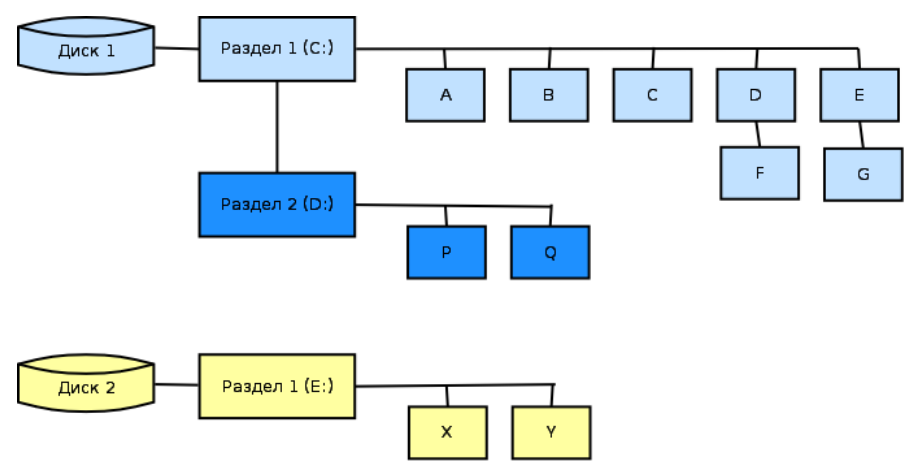
\includegraphics[scale=0.5]{images/lec09-pic01.png}
	\end{figure}
\end{frame}

\begin{frame}[fragile]{Пример структуры каталогов в Linux}
	\begin{figure}[h]
		\centering
		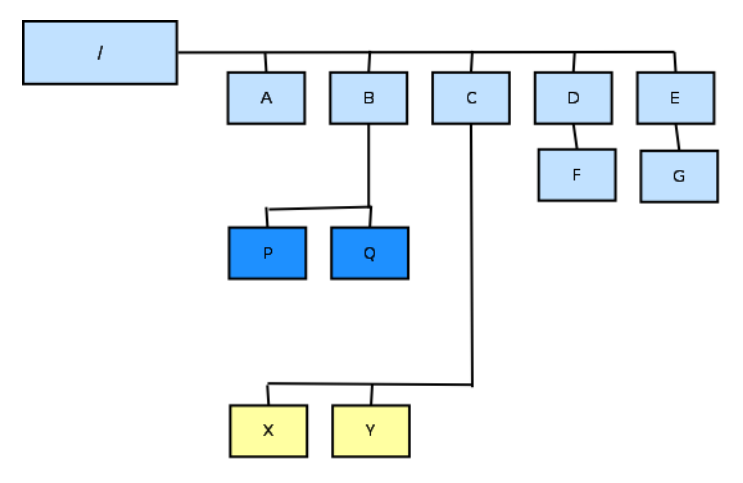
\includegraphics[scale=0.5]{images/lec09-pic02.png}
	\end{figure}
\end{frame}

\begin{frame}[fragile]{Дерево каталогов Linux}
Родительским для всех остальных каталогов является так называемый корневой каталог, обозначаемый <</>>.
	\begin{itemize}
		\item \textbf{/bin} -- основные системные утилиты, необходимые в однопользовательском режиме.
		\item \textbf{/boot} -- файлы загрузчика, например, образ ядра Linux.
		\item \textbf{/dev} -- файлы устройств.
		\item \textbf{/etc} -- общесистемные конфигурационные файлы и конфигурационные файлы программ.
		\item \textbf{/home} -- домашние каталоги пользователей. 
		\item \textbf{/lib} -- файлы общесистемных разделяемых библиотек и модулей ядра.
		\item \textbf{/media} -- точки монтирования для сменных носителей, таких как CD и DVD-диски, flash-накопители и т.п.
	\end{itemize}
\end{frame}

\begin{frame}[fragile]{Дерево каталогов Linux}
	\begin{itemize}
		\item \textbf{/mnt} -- точки монтирования для временных разделов.
		\item \textbf{/op}t -- дополнительные пакеты приложений.
		\item \textbf{/pro}c -- виртуальная файловую систему proc, которая отображает в виде структуры файлов и каталогов различную информацию о работе системы.
		\item \textbf{/root} -- домашний каталог пользователя root.
		\item \textbf{/sbi}n -- основные системные программы для администрирования и настройки системы.
		\item \textbf{/sys} -- точка монтирования еще одной виртуальной файловой системы sys, являющейся расширением proc.
		\item \textbf{/usr} -- содержит большинство пользовательских приложений и утилит, использующихся в многопользовательском режиме.
		\item \textbf{/va}r -- содержит изменяемые файлы, такие как файлы регистрации, временные файлы и т.п.		
	\end{itemize}
\end{frame}

\begin{frame}[fragile]{Служебные файловые системы}
	\begin{block}{Файловая система /dev}
		\begin{itemize}
			\item хранилище файлов символьных и блочных устройств.
		\end{itemize}
	\end{block}
	\begin{block}{Файловая система /proc}
		\begin{itemize}
			\item  была создана для предоставления пользователю информации о работающих процессах; 
			\item  затем туда стали помещать туда <<полезную>> информацию (версия ОС, объем оперативной памяти, сообщения ядра и т. п.);
			\item  в некоторые файлы дерева /proc можно писать, обеспечивая тем самым динамическое конфигурирование ядра.
		\end{itemize}
	\end{block}
	\begin{block}{Файловая система /tmp}
		\begin{itemize}
			\item предназначена для хранения временных файлов. 
			\item может располагаться как на диске, так и в памяти.
		\end{itemize}
	\end{block}
\end{frame}

\begin{frame}[fragile]
	\begin{block}{Монтирование файловых систем может выполняться:}		
		\begin{itemize}
			\item вручную администратором системы с помощью команды mount 
			\item автоматически при загрузке системы на основе файла настроек /etc/fstab		
		\end{itemize}
	\end{block}
	\begin{alltt}
		\$ mount
		/dev/sda2 on / type ext4 (rw)
		none on /proc type proc (rw)
		none on /proc/sys/fs/binfmt_misc type binfmt_misc (rw)
		/dev/sdb1 on /media/4779-86EA type vfat
		(rw,nosuid,nodev,uhelper=udisks,uid=500,gid=500,
		shortname=mixed,dmask=0077, utf8=1,flush)
	\end{alltt}
	DEVICE on MOUNTPOINT type FSTYPE (FLAGS)
	\begin{itemize}
		\item DEVICE — имя устройства.
		\item MOUNTPOINT — точка монтирования. 
		\item FSTYPE — тип файловой системы.
		\item FLAGS — опции монтирования. 
	\end{itemize}
\end{frame}

\section{Чтение информации о файловой системе}
\begin{frame}
  \frametitle{Содержание лекции}
  \tableofcontents[current]
\end{frame}

\begin{frame}[fragile]{Семейство statvfs()}
	\begin{block}{Информация о смонтированных файловых системах обычно хранится в файле/etc/mtab:}
		\begin{alltt}
			\$ cat /etc/mtab
			/dev/sda2 / ext4 rw 0 0
			none /proc proc rw 0 0
			none /proc/sys/fs/binfmt_misc binfmt_misc rw 0 0
		\end{alltt}
	\end{block}
	Каждая строка /etc/mtab соответствует одной смонтированной файловой системе и содержит шесть полей:
	\begin{itemize}
		\item Первое поле - носитель файловой системы.
		\item Второе поле - точка монтирования.
		\item Третье поле - тип файловой системы.
		\item Четвертое поле - флаги монтирования.
		\item Пятое поле используется утилитой суперпользователя dump.
		\item Шестое поле необходимо для утилиты fsck.
	\end{itemize}
\end{frame}


\begin{frame}[fragile]
	\begin{block}{Функции для разбора файла /etc/mtab:}
		\begin{minted}{c}
FILE * setmntent (const char * FILENAME, const char * MODE);
struct mntent * getmntent (FILE * FILEP);
int endmntent (FILE * FILEP);
		\end{minted} 
	\end{block}	
	\begin{itemize}
		\item \textit{setmntent}() открывает файл, в котором содержится список смонтированных файловых систем;
		\item \textit{getmntent}() извлекает следующую запись о файловой системе. 
		\item \textit{endmntent}() вызывается по окончании чтения записей о файловых системах.
	\end{itemize}
	Поля структуры \textit{mntent} соответствуют полям /etc/mtab:
	\begin{minted}{c}
	char *mnt_fsname;
	char *mnt_dir;
	char *mnt_type;
	char *mnt_opts;
	int mnt_freq;
	int mnt_passno;
	\end{minted}
\end{frame}

\begin{frame}[fragile]
	Более подробную информацию о файловых системах позволяют получить следующие функции, объявленные в заголовочном файле sys/statvfs.h:
	\begin{minted}{c}
int statvfs (const char * PATH, struct statvfs * FS);
int fstatvfs (int FD, struct statvfs * FS);
	\end{minted}
	\begin{itemize}
		\item \textit{f\_bsize} - целое число, содержащее размер блока файловой системы в байтах.
		\item \textit{f\_blocks} - целое число, показывающее количество блоков в файловой системе.
		\item \textit{f\_bfree} - целое число, содержащее количество свободных блоков в файловой системе.
		\item \textit{f\_bavail} содержит число доступных блоков, без учета резервных блоков, которые некоторые файловые системы выделяют для специального использования.
		\item \textit{f\_namemax} - целое число, показывающее максимально возможную длину имени файла в данной файловой системе. 
	\end{itemize}
\end{frame}

\begin{frame}[fragile]{Примеры}
\begin{block}{Пример 1. Работа функции statvfs()}
ex09\_01.c
\end{block}
\begin{block}{Пример 2. Работа функции fstatvfs()}
ex09\_02.c
\end{block}
\end{frame}

\section{Чтение каталогов}
\begin{frame}
  \frametitle{Содержание лекции}
  \tableofcontents[current]
\end{frame}

\begin{frame}[fragile]{Текущий каталог: getcwd()}
	Каждый дочерний процесс наследует от своего родителя независимую копию текущего каталога.

	Для получения значения текущего каталога используется системный вызов \textbf{getcwd}(), объявленный в заголовочном файле \textit{unistd.h} следующим образом:
	\begin{minted}{c}
	char * getcwd (char * BUFFER, size_t SIZE);
	\end{minted}
	Чтобы получить только базовое имя каталога, можно воспользоваться функцией \textbf{basename}(), объявленной в заголовочном файле \textit{string.h} следующим образом:
	\begin{minted}{c}
	char * basename (const char * PATH);
	\end{minted}
	\begin{block}{Примеры. Получение текущего каталога}
		ex09\_03.c, ex09\_04.c
	\end{block}
\end{frame}

\begin{frame}[fragile]{Смена текущего каталога: chdir()}
	Любой процесс может сменить свой текущий каталог. Это можно сделать при помощи одного из приведенных далее системных вызовов, объявленных в заголовочном файле \textit{unistd.h}:
	\begin{minted}{c}
	int chdir (const char * PATH);
	int fchdir (int FD);
	\end{minted}
	\begin{itemize}
		\item Обе функции возвращают \textbf{0} при успешном завершении и \textbf{–1}, если произошла ошибка. 
		\item Системный вызов \textit{chdir}() изменяет текущий каталог, используя его имя (путь), а \textit{fchdir}() вместо имени читает файловый дескриптор каталога.
	\end{itemize}
	\begin{block}{Примеры. Смена текущего каталога}
		ex09\_05.c, ex09\_06.c
	\end{block}
\end{frame}

\begin{frame}[fragile]{Открытие и закрытие каталога}
	Пользовательские библиотеки располагаются на верхнем уровне реализации файловой системы, каталог здесь рассматривается как самостоятельная сущность, не являющаяся особым файловым типом. 
	\begin{itemize}
		\item В стандартной библиотеке языка C абстракцией каталога является указатель типа \textbf{DIR}. 
		\item Прежде чем читать содержимое каталога, его нужно открыть, а прочитанный каталог полагается закрывать.
	\end{itemize}
	\begin{minted}{c}
	DIR * opendir (const char * NAME);
	int closedir (DIR * DIRP);
	DIR * fdopendir (int FD);
	\end{minted}
	\begin{itemize}
		\item Первая функция открывает каталог с именем \textbf{NAME} и возвращает указатель типа \textbf{DIR}. В случае ошибки возвращается \textbf{NULL}. 
		\item Функция \textit{closedir}() закрывает каталог и возвращает \textbf{0} при успешном завершении, в случае ошибки \textbf{–1}
\end{itemize}
\end{frame}

\begin{frame}[fragile]{Чтение каталога: readdir()}
	Для чтения содержимого каталога применяется функция \textbf{readdir}(), объявленная в заголовочном файле \textit{dirent.h} следующим образом:
	\begin{minted}{c}
	struct dirent * readdir (DIR * DIRP);
	\end{minted}
	Структура dirent содержит несколько полей, но нам понадобится только одно из них:
	\begin{minted}{c}
	struct dirent {
	  /* ... */
	  char * d_name;
	};
	\end{minted}
	Функция \textit{readdir}() заносит в поле \textbf{d\_name} структуры \textbf{dirent} имя очередного элемента просматриваемого каталога. Если каталог полностью просмотрен, то \textit{readdir}() возвращает \textbf{NULL}.
	\begin{block}{Примеры. Просмотр каталога}
		ex09\_07.c
	\end{block}
\end{frame}

\begin{frame}[fragile]{Получение данных о файлах: семейство stat()}
	Дополнительную информацию о файлах позволяют получить системные вызовы семейства stat(), объявленные в заголовочном файле sys/stat.h:
	\begin{minted}{c}
int stat (const char * FNAME, struct stat * STATISTICS);
int fstat (int FD, struct stat * STATISTICS);
int lstat (const char * FNAME, struct stat * STATISTICS);
	\end{minted}
	\begin{itemize}
		\item Системный вызов \textbf{stat}() читает информацию о файле с именем \textbf{FNAME} и записывает эту информацию в структуру \textbf{stat} по адресу \textbf{STATISTICS}. 
		\item Вызов \textbf{fstat}() также читает информацию о файле, который представлен дескриптором \textbf{FD}. 
		\item \textbf{lstat}() работает аналогично \textbf{stat}(), но при обнаружении символической ссылки \textbf{lstat}() читает информацию о ней, а не о файле, на который эта ссылка указывает.
	\end{itemize}
\end{frame}

\begin{frame}[fragile]
	Структура \textbf{stat} также объявлена в файле \textit{sys/stat.h}. Для нас наибольший интерес представляют следующие поля этой структуры:
	\begin{minted}{c}
	struct stat{
	  /* режим файла */
	  mode_t st_mode; 
	  /* числовой идентификатор владельца файла */
	  uid_t st_uid; 
	  /* идентификатор группы */
	  gid_t st_gid; 
	  /* размер файла в байтах */
	  off_t st_size; 
	  /* дата и время последнего обращения к файлу */
	  time_t st_atime; 
	  /* дата и время последней модификации файла */
	  time_t st_mtime; 
	};
	\end{minted}
\end{frame}

\begin{frame}[fragile]{Примеры}
	\begin{block}{Пример 8. Системный вызов stat()}
		ex09\_08.c
	\end{block}
	\begin{block}{Пример 9. Системный вызов fstat()}
		ex09\_09.c
	\end{block}
	\begin{block}{Пример 10. Системный вызов lstat() }
		ex09\_10.c
	\end{block}
\end{frame}

\begin{frame}[fragile]{Биты режима файла}
	Биты режима файла делятся на три группы:
	\begin{itemize}
		\item базовые права доступа;
		\item расширенные права доступа;
		\item тип файла.
	\end{itemize}
	Проверка базовых прав доступа: сравнить режим файла (\textbf{st\_mode} структуры \textbf{stat}) с одной из констант из \textit{sys/types.h} (S\_IRUSR, S\_IWUSR и т. п.) с использованием операции побитовой конъюнкции (И).
	\begin{minted}{c}
	mode & S_IWUSR //владельцу разрешено писать в файл
	\end{minted}
	Проверка расширенных прав доступа:
	\begin{itemize}
		\item S\_ISUID - установка и проверка бита SUID;
		\item константа S\_ISGID установка и проверка бита SGID;
		\item константа S\_ISVTX установка и проверка sticky-бита.
	\end{itemize}
\end{frame}

\begin{frame}[fragile]{Биты режима файла}
	Для определения типа файла применяются следующие макросы::
	\begin{itemize}
		\item S\_ISDIR(mode) - каталог;
		\item S\_ISCHR(mode) - символьное устройство;
		\item S\_ISBLK(mode) - блочное устройство;
		\item S\_ISREG(mode) - обычный файл;
		\item S\_ISFIFO(mode) - именованный канал FIFO;
		\item S\_ISLNK(mode) - символическая ссылка;
		\item S\_ISSOCK(mode) - сокет.
	\end{itemize}
	\begin{block}{Пример. Чтение содержимого каталога}
		ex09\_11.c
	\end{block}
\end{frame}

\begin{frame}[fragile]{Чтение ссылок}
Программа \textbf{ls}, вызванная с флагом \textbf{–l}, позволяет узнать, на какой файл указывает символическая ссылка:
	\begin{alltt}
		\$ touch myfile
		\$ ln -s myfile mylink
		\$ ls -l mylink
		lrwxrwxrwx 1 nnivanov nnivanov 6 2011-05-07 
		                     09:59 mylink -> myfile
	\end{alltt}
	Такая операция называется разыменованием символической ссылки (\textit{symlink dereferencing}) или разрешением имени файла (\textit{filename resolution}).
\end{frame}

\begin{frame}[fragile]{Чтение ссылок}
	Разыменование символических ссылок осуществляется при помощи системного вызова \textbf{readlink}(), который объявлен в заголовочном файле \textit{unistd.h} следующим образом:
	\begin{minted}{c}
	ssize_t readlink (const char * SYMLNK, char * BUF, 
    	size_t SIZE);
	\end{minted}
	\begin{itemize}
		\item системный вызов помещает в буфер \textbf{BUF} размера \textbf{SIZE} путь к файлу, на который указывает символическая ссылка \textbf{SYMLNK}. 
		\item Возвращаемое значение -- число байтов, записанных в буфер \textbf{BUF}. В случае ошибки возвращается \textbf{–1}.
		\item \textit{readlink}() не завершает буфер нультерминатором.
	\end{itemize}
	\begin{block}{Пример. Чтение ссылок}
		ex09\_12.c
	\end{block}
\end{frame}

\section{Операции над файлами}

\subsection{Удаление файла}

\begin{frame}[fragile]{Удаление файла: unlink()}
	Для удаления файла служит системный вызов \textbf{unlink}(), объявленный в заголовочном файле \textit{unistd.h} следующим образом:
	\begin{minted}{c}
	int unlink (const char * FNAME);
	\end{minted}
	\begin{itemize}
		\item Аргумент \textbf{FNAME} — это имя удаляемого файла. 
		\item \textit{unlink}() возвращает \textbf{0} при успешном завершении. 
		\item В случае ошибки возвращается \textbf{–1}.
	\end{itemize}
\end{frame}

\begin{frame}[fragile]{Удаление файла: unlink()}
	\begin{minted}{c}
#include <stdio.h>
#include <unistd.h>

int main (int argc, char ** argv)
{
  if (argc < 2) return 1;
  
  if (unlink (argv[1]) == -1) {
   	fprintf (stderr, "Cannot unlink file (\%s)", 
   	  argv[1]);
   	return 1;
  }
  
  return 0;
}
	\end{minted}
\end{frame}

\begin{frame}
	\begin{block}{Файл}
		комплексное понятие, состоящее из следующих компонентов:
		\begin{itemize}
			\item данные (data);
			\item индексы (inodes);
			\item ссылки (links).
		\end{itemize}
	\end{block}
	\begin{block}{Индексы}
		специальные ячейки памяти, зарезервированные файловой системой для разделения данных на файлы. 
	\end{block}
	\begin{itemize}
		\item Каждый индекс имеет уникальный (в рамках данной файловой системы) номер.
		\item Индексы содержат информацию о том, в каких блоках файловой системы хранятся данные конкретного файла. 
		\item В индексах содержатся сведения о дате и времени открытия и модификации файла. 
		\item Ссылка - имя индексного узла файловой системы. 
	\end{itemize}
\end{frame}

\begin{frame}[fragile]{Индексы}
	Программа \textbf{ls}, вызванная с флагом \textbf{-i}, позволяет увидеть номер индексного узла, на который указывает ссылка:
	\begin{alltt}
		\$ mkdir idemo
		\$ cd idemo
		\$ touch file1
		\$ touch file2
		\$ ls -i

		952139 file1 
		952141 file2
	\end{alltt}
	\begin{itemize}
		\item \textit{file1} — это ссылка на индекс с номером 952139 
		\item \textit{file2} указывает на другой индексный узел с номером 952141
	\end{itemize}
\end{frame}

\begin{frame}[fragile]{Индексы}
	Продолжим:
	\begin{alltt}
		\$ ln -s file1 symlnkf1
		\$ ls -i

		952139 file1 
		952141 file2 
		952190 symlnkf1
	\end{alltt}
	\begin{itemize}
		\item символическая ссылка является также ссылкой на индекс с номером 952190
		\item символические ссылки указывают не на индекс, а на имя файла
	\end{itemize}
\end{frame}

\begin{frame}[fragile]{Индексы}
	Теперь воспользуемся командой \textbf{ln} без флага \textbf{-s}:
	\begin{alltt}
		\$ ln file1 hardfile1
		\$ ls -i

		952139 file1 952141 file2 952139 hardfile1 952190 symlnkf1
	\end{alltt}
	\begin{itemize}
		\item \textit{hardfile1} является жесткой ссылкой на файл \textit{file1}. Вывод команды \textit{ls} показывает, что \textit{file1} и \textit{hardfile1} указывают на один и тот же индекс с номером 952139. 
		\item жесткие ссылки (в отличие от символических) не носят подчиненный характер. \textit{file1} и \textit{hardfile1} — это полноценные ссылки на один и тот же индексный узел.
	\end{itemize}
\end{frame}

\begin{frame}[fragile]{Индексы}
	Если две ссылки указывают на один и тот же индекс, то можно сказать, что они имеют доступ к одним и тем же данным:
	\begin{alltt}
		\$ echo hello > file1
		\$ cat hardfile1
		hello
	\end{alltt}
	Индексы являются промежуточным звеном, связывающим ссылку с данными на блочном устройстве. 
\end{frame}

\begin{frame}[fragile]{Команда rm}
	Программа \textbf{rm} работает следующим образом:
	\begin{itemize}
		\item если удаляемый файл является последней ссылкой на соответствующий индексный узел в файловой системе, то данные и индекс 		освобождаются;
		\item если в файловой системе еще остались ссылки на соответствующий индексный узел, то удаляется только ссылка.
	\end{itemize}
	\begin{alltt}
		\$ rm file1
		\$ cat hardfile1
		hello
	\end{alltt}
	
	Теперь обратите внимание на вывод программы \textbf{ls} с флагом \textbf{-l}:
	\begin{alltt}
		\$ ls -l
		-rw-r--r-- 1 kt kt 0 2011-05-07 10:00 file2
		-rw-r--r-- 1 kt kt 6 2011-05-07 10:00 hardfile1
		lrwxrwxrwx 1 kt kt 5 2011-05-07 10:00 symlnkf1 -> file1
	\end{alltt}
\end{frame}

\begin{frame}[fragile]{Команда rm}
	Символическая ссылка \textit{symlnkf1} по-прежнему указывает на файл \textit{file1}, которого уже не существует:
	\begin{alltt}
		\$ cat symlnkf1
		cat: symlnkf1: No such file or directory
	\end{alltt}
	Числа во втором столбце вывода программы \textbf{ls} - счетчики ссылок на соответствующие индексные узлы.
	\begin{alltt}
		\$ ls -l
		-rw-r--r-- 2 kt kt 0 2011-05-07 10:00 file2
		-rw-r--r-- 1 kt kt 6 2011-05-07 10:00 hardfile1
		-rw-r--r-- 2 kt kt 0 2011-05-07 10:00 hardfile2
		lrwxrwxrwx 1 kt kt 5 2011-05-07 10:00 symlnkf1 -> file1
	\end{alltt}
\end{frame}

\begin{frame}[fragile]{Команда df}
	Если вызвать команду \textbf{df} с флагом \textbf{-i}, то на экран будет выведена информация по индексным узлам смонтированных файловых систем:
	\begin{alltt}
		\$ df -i

		Filesystem Inodes IUsed IFree IUse\% Mounted on
		/dev/sda6 1311552 264492 1047060 21\% /
		udev 96028 487 95541 1\% /dev
		/dev/sda1 66264 58 66206 1\% /boot
		/dev/sda7 3407872 149600 3258272 5\% /home
	\end{alltt}
	В файловых системах может присутствовать ограниченное число индексов (столбец \textbf{Inodes}). Столбец \textbf{IUsed} показывает число используемых индексов, а в столбце \textbf{IFree} содержится число свободных индексных узлов файловой системы
\end{frame}

\begin{frame}[fragile]{Команда df}
	Каждый раз при создании файла в файловой системе выделяется индекс:
	\begin{alltt}
		\$ df -i .
		Filesystem Inodes IUsed IFree IUse\% Mounted on
		/dev/sda7 3407872 149586 3258286 5\% /home

		\$ touch file3
		\$ df -i .

		Filesystem Inodes IUsed IFree IUse\% Mounted on
		/dev/sda7 3407872 149587 3258285 5\% /home
	\end{alltt}
\end{frame}

\begin{frame}[fragile]{Команда df}
	Создание жесткой ссылки не приводит к появлению в файловой системе нового индекса:
	\begin{alltt}
		\$ df -i .
		Filesystem Inodes IUsed IFree IUse\% Mounted on
		/dev/sda7 3407872 149587 3258285 5\% /home

		\$ ln file3 hardfile3
		\$ df -i .
		Filesystem Inodes IUsed IFree IUse\% Mounted on
		/dev/sda7 3407872 149587 3258285 5\% /home
	\end{alltt}
\end{frame}

\begin{frame}[fragile]{Пример statvfsinode.c}
	В рассматриваемом ранее примере программа использовала функцию \textbf{statvfs}() для вывода информации о смонтированных файловых системах. 

	Структура \textit{statvfs} содержит также следующие поля, которые мы не рассматривали:
	\begin{itemize}
		\item f\_files — общее число индексов для данной файловой системы;
		\item f\_free — число свободных индексов файловой системы;
		\item f\_favail — число доступных индексов в файловой системе.
	\end{itemize}
\end{frame}

\begin{frame}[fragile]{Пример statinode.c}
	Структура \textbf{stat} содержит еще одно поле st\_ino, в котором находится номер индексного узла, на который ссылается файл.
	\begin{minted}{c}
    struct stat st;
    if (stat(argv[1], &st) == -1) {
        fprintf (stderr, "stat() error\n");
        return 1;
    }
    printf ("FILE:\t\t%s\n", argv[1]);
    printf ("UID:\t\t%d\n", (int) st.st_uid);
    printf ("GID:\t\t%d\n", (int) st.st_gid);
    printf ("SIZE:\t\t%ld\n", (long int) st.st_size);
    printf ("AT:\t\t%s", ctime (&st.st_atime));
    printf ("MT:\t\t%s", ctime (&st.st_mtime));
    printf ("INODE:\t\t%ld\n", (long int) st.st_ino);
	\end{minted}
\end{frame}

\begin{frame}[fragile]
	Cистемный вызов unlink() (unlink2.c) удаляет ссылку на индексный узел. Если эта ссылка была последней, то индекс освобождается.
	\begin{alltt}
		\$ touch file1
		\$ ln file1 file2
		\$ ls -i file1 file2
		1048740 file1 1048740 file2
		\$ ./unlink2 file1
		\$ ls file1
		/bin/ls: file1: No such file or directory
		\$ cat file2
		Hello World
	\end{alltt}
	Над открытым файлом можно успешно осуществлять операции ввода-вывода, даже если последняя ссылка на этот файл удалена:
	\begin{alltt}
		\$ ./unlink2 file2
		\$ ls file2
		/bin/ls: file2: No such file or directory
	\end{alltt}
\end{frame}

\subsection{Перемещение файла}

\begin{frame}[fragile]{Перемещение файлов}
	Системный вызов rename() позволяет переименовывать или перемещать файл в пределах одной файловой системы.
	\begin{minted}{c}
	int rename (const char * OLDF, const char * NEWF);
	\end{minted}
	\begin{itemize}
		\item При успешном завершении rename() возвращает 0. 
		\item В случае ошибки возвращается –1
	\end{itemize}
	Пример (rename1.c):
	\begin{minted}{c}
    if (rename (argv[1], argv[2]) == -1) {
        fprintf (stderr, "rename() error\n");
        return 1;
    }    
	\end{minted}
\end{frame}

\begin{frame}[fragile]{Перемещение файлов: rename2.c}
	Теперь проведем небольшой эксперимент:
	\begin{alltt}
		\$ touch file1
		\$ cat file1
		\$ ./rename2 file1 file2
		\$ ls file1
		/bin/ls: file1: No such file or directory
		\$ cat file2
		Hello World
	\end{alltt}
	Перемещение открытого файла никак не отражается на операциях ввода-вывода.
\end{frame}

\subsection{Создание ссылок}

\begin{frame}[fragile]{Создание ссылок}
	Ссылки в файловой системе Linux бывают двух типов:
	\begin{itemize}
		\item символические ссылки (\textit{symbolic links});
		\item жесткие (прямые) ссылки (\textit{hard links}).
	\end{itemize}
	В распоряжении программиста имеются следующие системные вызовы:
	\begin{minted}{c}
int link (const char * FROM, const char * TO);
int symlink (const char * FROM, const char * TO);
	\end{minted}
	Оба вызова возвращают \textbf{0} при успешном завершении и \textbf{–1}, если произошла ошибка.
	Примеры: 
	\begin{itemize}
		\item linkdemo.c
		\item symlinkdemo.c
	\end{itemize}
\end{frame}

\subsection{Создание и удаление каталогов}

\begin{frame}[fragile]{Создание каталога}
	Для создания каталога используется системный вызов \textbf{mkdir}():
	\begin{minted}{c}
	int mkdir (const char * NAME, mode_t MODE)
	\end{minted}
	Системный вызов \textit{mkdir}() создает каталог с именем \textbf{NAME} и режимом \textbf{MODE}. При успешном завершении \textit{mkdir}() возвращает \textbf{0}. В случае ошибки возвращается \textbf{–1}. Примеры: 
	\begin{itemize}
		\item mkdir1.c
		\item mkdir2.c
	\end{itemize}
\end{frame}

\begin{frame}[fragile]{Создание каталога}
	Программа mkdir работает не так, как мы ожидали:
	\begin{alltt}
		\$ ./mkdir2 mydir
		\$ ls -l | grep mydir
		drwxr-xr-x 2 kt kt 4096 2011-05-07 10:09 mydir
	\end{alltt}
	В системный вызов \textit{mkdir}() передавался аргумент \textbf{mode}, в котором все биты базовых прав доступа установлены в единицу. Но вывод программы \textbf{ls} показывает, что созданный каталог имеет права доступа \textbf{0755}.
\end{frame}

\begin{frame}[fragile]
	К каждому процессу в \textit{Linux} привязана маска прав доступа, которая наследуется потомком от родительского процесса (аналогично текущему каталогу, окружению и т. п.). 
	\begin{block}{Маска прав доступа}
		число, представляющее собой набор битов прав доступа, которые никогда не будут устанавливаться для создаваемых процессом файлов или 	каталогов.
	\end{block}
	Команда \textbf{umask} позволяет узнать текущую маску прав доступа командной оболочки:
	\begin{alltt}
		\$ umask
		0022
	\end{alltt}
	Маска прав доступа \textbf{0022} разрешает при создании файлов или каталогов устанавливать любые права доступа для владельца, но не разрешает права на запись для группы и остальных пользователей.
\end{frame}

\begin{frame}[fragile]{Маски прав доступа}
	Текущий процесс вправе изменять свою копию маски прав доступа:
	\begin{alltt}
		\$ umask 0044
		\$ umask
		0044
	\end{alltt}
	Дочерние процессы наследуют копию маски прав доступа родительского процесса:
	\begin{alltt}
		\$ umask 000
		\$ umask
		0000
		\$ bash
		\$ umask
		0000
		\$ exit
		exit
	\end{alltt}
\end{frame}

\begin{frame}[fragile]{Создание каталога}
	Попробуем запустить программу \textit{mkdir2} с измененной маской прав доступа оболочки:
	\begin{alltt}
		\$ umask 0000
		\$ umask
		0000
		\$ ./mkdir2 mydir
		\$ ls -l | grep mydir
		drwxrwxrwx 2 kt kt 4096 2011-05-07 10:15 mydir
	\end{alltt}
\end{frame}

\begin{frame}[fragile]{Системный вызов umask()}
	Программа может изменить маску прав доступа текущего процесса при помощи системного вызова \textbf{umask}():
	\begin{minted}{c}
	mode_t umask (mode_t MASK);
	\end{minted}
	Этот системный вызов изменяет текущую маску прав доступа и возвращает предыдущее значение маски.
	Примеры: 
	\begin{itemize}
		\item mkdir3.c
	\end{itemize}
	\begin{alltt}
		\$ umask 0022
		\$ umask
		0022
		\$ ./mkdir3 mydir
		\$ ls -l | grep mydir
		drwxrwxrwx 2 kt kt 4096 2011-05-07 10:17 mydir
	\end{alltt}
\end{frame}

\begin{frame}[fragile]{Создание каталога}
	Пример создания каталога с <<липким битом>>:  
	\begin{itemize}
		\item mkdir4.c
	\end{itemize}
	\begin{alltt}
		\$ ./mkdir4 mydir
		\$ ls -l | grep mydir
		drwxrwxrwt 2 kt kt 4096 2011-05-07 10:20 mydir
	\end{alltt}
\end{frame}

\begin{frame}[fragile]{Удаление каталога}
	Для удаления каталога служит системный вызов \textbf{rmdir}():
	\begin{minted}{c}
	int rmdir (const char * DIR)
	\end{minted}
	\begin{itemize}
		\item Аргумент \textbf{DIR} — это имя (путь) к каталогу, который следует удалить.
		\item При успешном завершении \textit{rmdir}() возвращает \textbf{0}. В случае ошибки возвращается \textbf{–1}. 
	\end{itemize}
	Пример: 
	\begin{itemize}
		\item rmdirdemo.c
	\end{itemize}
	Системный вызов \textit{rmdir}() удаляет только пустые каталоги. Если каталог не пуст, то \textit{rmdir}() завершится неудачей.
\end{frame}

\end{document}